\documentclass[tikz]{standalone}

\usepackage{tikz}
\usetikzlibrary{trees}
\usetikzlibrary{shapes}
\usetikzlibrary{positioning}
\usetikzlibrary{arrows.meta}

\tikzset{
    mynode/.style = {circle, ultra thick, draw=black, align=center,fill=yellow!30,font=\ttfamily\bfseries\Large,text=black},
    mynoder/.style = {circle, ultra thick, draw=black, align=center,fill=red!30,font=\ttfamily\bfseries\Large,text=black},
    mynodeb/.style = {circle, ultra thick, draw=black, align=center,fill=blue!30,font=\ttfamily\bfseries\Large,text=black},
    mynodeg/.style = {circle, ultra thick, draw=gray, align=center,fill=gray!05,font=\ttfamily\bfseries\Large,text=gray!20},
    mynodegr/.style = {circle, ultra thick, draw=gray, align=center,fill=gray!05,font=\ttfamily\bfseries\Large,text=red},
    edgen/.style = {-,ultra thick,black},
    edger/.style = {-,ultra thick,red},
    edgeb/.style = {-,ultra thick,blue},
    edgeg/.style = {-,ultra thick,gray},
    edgegd/.style = {-,ultra thick,brown,dashed}, % back
    edgevd/.style = {-,ultra thick,violet,dotted}, % forward
    edgexd/.style = {-,ultra thick,blue,densely dotted}, % traversal
    every picture/.style={/utils/exec={\ttfamily\bfseries}},
    every picture/.style={font issue=\ttfamily\bfseries},
    font issue/.style={execute at begin picture={#1\selectfont}}
}

\begin{document}

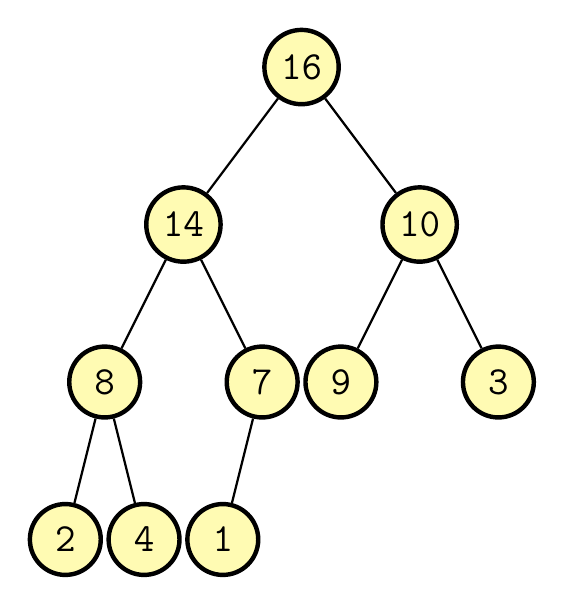
\begin{tikzpicture}[
	thick,
	level distance=2cm,
  level 1/.style={sibling distance=3cm},
  level 2/.style={sibling distance=2cm},
  level 3/.style={sibling distance=1cm},
	font=\ttfamily\bfseries]
  \node[mynode, minimum size=0.9cm] {16}
    child {node[mynode, minimum size=0.9cm] {14}
      child {node[mynode, minimum size=0.9cm] {8}
        child {node[mynode, minimum size=0.9cm] {2}}
        child {node[mynode, minimum size=0.9cm] {4}}
      }
      child {node[mynode, minimum size=0.9cm] {7}
        child {node[mynode, minimum size=0.9cm] {1}}
        child[missing] {node[mynode, minimum size=0.9cm] {}}
      }
    }
    child {node[mynode, minimum size=0.9cm] {10}
      child {node[mynode, minimum size=0.9cm] {9}
      }
      child {node[mynode, minimum size=0.9cm] {3}
      }
    };
\end{tikzpicture}

\end{document}